\documentclass{article} % For LaTeX2e
\usepackage{iclr2017_conference,times}
%\usepackage{hyperref}
\usepackage{url}
\usepackage{amsthm}
\usepackage{times}
\usepackage{graphicx}
\usepackage{color}
\usepackage{amsmath}
\usepackage{amsfonts}
\usepackage{url}
\usepackage{textcomp}
\usepackage{amsthm}
\usepackage{float}

\frenchspacing

\def\presentationmode{1}

\def\beginFrame#1{\if\presentationmode1 \begin{frame}{#1} \else \fi}
\def\endFrame{\if\presentationmode1 \end{frame} \else \fi}

\newcommand{\mat}[1]{\mathrm{\mathbf{#1}}}
\newcommand{\vect}[1]{\mathrm{\mathbf{#1}}}
\newcommand{\fros}[1]{\left\| #1 \right\|_\mathrm{F}^2}
\newcommand{\Expect}[2]{\mathbb{E}_{#1}\left[ #2 \right]}
\newcommand{\KL}[2]{ \mathrm{KL}\left( #1 \| #2 \right) }
\newcommand{\Real}{\mathbb{R}}
\newcommand{\T}{\mathrm{T}}
\newcommand{\tr}{\mathrm{tr}}
\newcommand{\sigmoid}{\sigma}
\newcommand{\attention}{\vect{g}}
\def\attentionwithouti{g_2, \dots, g_k}
%\def\attentionwithouti{\boldsymbol{\gamma}_{i}}
\newcommand{\attraction}{\vect{h}}

\def\x{\vect{x}}
\def\y{\vect{y}}
\def\h{\vect{h}}
\def\g{\vect{g}}
\def\s{\vect{s}}
\def\c{\vect{c}}
\def\A{\mathcal{A}}
\def\S{\mathcal{S}}
\def\R{\mathcal{R}}
\def\Trans{\mathcal{T}}
\def\Observations{\Omega}
\def\ObProb{\mathcal{O}}
\def\E{\mathcal{E}}
\def\deriv#1#2{ \frac{\partial #2}{ \partial #1 } }
\def\derivN#1#2#3{ \frac{\partial^{#1} #3}{ \partial #2^{#1} } }
\def\grad#1#2{ \deriv{#1}{#2} }
\def\gradN#1#2#3{ \derivN{#1}{#2}{#3} }
\def\Grad#1#2{ \nabla_{#1} {#2} }
\def\obs{\vect{o}}
\def\u{{\boldsymbol{b}}}
\def\w{{\boldsymbol{\alpha}}}
\def\vmu{{\boldsymbol{\mu}}}
\def\v{\vect{v}}
\def\g{\attention}
\def\h{\attraction}
\def\G{\mat{G}}
\def\op{}
%\def\Qg{Q^{\mathrm{g}}}
%\def\ug{\vect{u}^{\mathrm{g}}}
\def\Qg{Q}
\def\ug{\u}
\def\params{{\boldsymbol{\theta}}}
\def\Params{{\boldsymbol{\Theta}}}
\def\opt#1{{\hat{#1}}}

\newcommand{\argmax}{\mathop{\rm argmax}\limits}
\newcommand{\argmin}{\mathop{\rm argmin}\limits}


%\def\costof#1{C(#1)}
\def\costof#1{\mathrm{C}[{#1}]}
\def\budget{B}
\def\cost{c}
\def\vcost{\vect{\cost}}
\def\costat#1{\cost_{#1}}
\def\costi{c_i}
\def\unit{\vect{e}}
\def\state{\s}
\def\action{a}
\def\rewards{y}

\def\sumk#1{\sum_{#1=1}^k}
\def\Si{\sumk{i}}
\def\Sj{\sumk{j}}

\def\vcatout{\tilde{\vect{h}}}
\def\catout{\tilde{h}_i}
\def\catoutj{\tilde{h}_j}
\def\changeof#1{\Delta #1}

\def\vcatin{\vect{h}}
\def\catin{h_{i}}
\def\catinj{h_{j}}

\def\vcatbias{\vect{h}_i}
\def\catbias{\mu_i}
\def\catbiasj{\mu_j}

\def\qbias{q_i}
\def\vqbias{\mathbf{q}}
\def\qin{Q}

\def\ebias{e_{-i}}
\def\ein{e}
\def\changeofebias{{\changeof\qbias} \left[ \changeof\qbias + 2 \TDerror{\qin} \right]}
%\def\changeofebias{{\changeof\qbias}\left( \changeof\qbias + 2 \delta_t \right)}

\def\regret{\rho_{-i}}
%\def\TDerror#1{E_{\mathrm{TD}}\left({#1}\right)}
\def\TDerror#1{\delta}


\def\prA{p(\rewards|\state, \action, \params, \g)}
\def\LLAttention{\log \prA}

\def\Square#1{\left[ #1 \right]^2}

\def\ReplayMemory{\mathcal{D}}
\def\play{\s_t, a_t, r_t, \s_{t+1}}
\def\Play{(\play)}
\def\pl{\mathsf{d}_t}
\def\Replays#1{\Expect{ \pl \sim \ReplayMemory}{#1}}

\def\bUpdate#1{p(o_{t+1}|s_${#1},a_t) \sum_i p(s_{#1}|s_i, a_t) b_{t}^i}
\def\beliefState#1{ \vect{b}_{#1} }

\def\const{\mathrm{const.}}
\def\test{_\mathrm{test}}
\def\train{_\mathrm{train}}
\def\bs{\boldsymbol}
\def\etal#1{{et al.} (\citeyear{#1})}
\def\Etal{{et al.}}
\def\Long{1}
\def\eg{e.g., }

\def\eAt#1{e_{#1}}
\def\eBase{\eAt{\one}}
\def\one{\mathbf{1}}
\def\zero{\mathbf{0}}
\def\unit#1{\vect{u}_{#1}}
\def\eChange#1{ \Delta e_{#1} }

\def\ask{q}


% probability
\def\prob#1{p\left(#1\right)}
\def\prob#1#2{p\left(#1 \mid #2 \right)}

\def\deprecated{\alert{[Deprecated]}}
\def\softmax{\mathrm{softmax}}


\newcommand{\penalvec}[3]{ \frac{1}{2 \sigma_#1^2} \sum_{#2=1}^{#3} \vect{#1}_{#2}^\T  \vect{#1}_{#2} }

\newcommand{\CON}{\color{red}}
%\newcommand{\CON}{\color{black}}
\newcommand{\COFF}{\color{black}}

%\newcommand{\CON}{\color{red} -------- My modification starts from here. ------- \color{black}}
%\newcommand{\CON}{\color{black}}
%\newcommand{\COFF}{\color{red} -------- My modification ends here. ------- \color{black} }


\newtheorem{thm}{Theorem}[section]
\newtheorem{coro}{Corollary}[section]
\newtheorem{prf}{Proof}
\newtheorem{defn}{Definition}




%=================================
% Paper specific
%=================================

\def\neuralnet{\mathfrak{G}}
\def\units{\mathcal{V}}
\def\edges{\mathcal{E}}
\def\unitAt#1{v_{#1}}
\def\unit{\unitAt{i}}
\def\followees{N^\mathrm{in}_i}
\def\followers{N^\mathrm{out}_i}
\def\friends{N_i}
\def\rewardAt#1{R_{#1}}
\def\reward{\rewardAt{it}}



%\title{Representation Market: Towards Model Aggregation on Decentralized Environment}
\title{Neuron as an Agent}

\author{Shohei Ohsawa \\
The University of Tokyo\\
7 Chome-3-1 Hongo, Bunkyo, Tokyo \\
\texttt{ohsawa@weblab.t.u-tokyo.ac.jp} \\
}

% The \author macro works with any number of authors. There are two commands
% used to separate the names and addresses of multiple authors: \And and \AND.
%
% Using \And between authors leaves it to \LaTeX{} to determine where to break
% the lines. Using \AND forces a linebreak at that point. So, if \LaTeX{}
% puts 3 of 4 authors names on the first line, and the last on the second
% line, try using \AND instead of \And before the third author name.

\newcommand{\fix}{\marginpar{FIX}}
\newcommand{\new}{\marginpar{NEW}}

%\iclrfinalcopy % Uncomment for camera-ready version

\begin{document}


\maketitle

\begin{abstract}
The reason why swarm of agents solve real-world problem well is, interestingly,
same as the principle of representation learning: good representation improves
perforamance of machine learning. Most of the problem in real-world is not
Markov decision process (MDP) but partially observed MDP (POMDP). On the
POMDP environment, good observation yields good action. In this paper, we
optimise a deep neural network as a multi-agent system as a natural extension
from representation learning to multi-agent reinforcement learning for POMDP.
To achieve that, we propose a novel learning framework, neuron as an agent
(NaaA). In NaaA, an individual unit is considered as an agent, and they maximizing
profit instead of minimizing error. To prevent dillemma, we borrow idea
from machanism design, ka field of game theory. To this end, we show all the unit
have valid price reflecting their contribution to performance at convergence. We
confirm the result by numerical experiment using Atari and VizDoom.
\end{abstract}

\section{Introduction}
% ・多分一回 MTG した方がいい(ストーリーの作り方、トピックセンテンス)
% ・有用な観測に対してインセンティブを与える
% ・高次のニューロンも、見方によっては下位のニューロンの信号を観測するメタセンサーであると考えられる 
% このあたりはまだストーリー作りできていません。

マルチエージェントによる強化学習が現実の課題に対して有効である理由は、興味深いことに表現学習の原理と一致する:有用な表現は予測性能を向上させる。
現実にある問題の多くは、DQN が前提としているマルコフ決定過程(MDP)ではなく部分的観測マルコフ決定過程(POMDP)である\citep[p.258]{sutton1998reinforcement}。
POMDP において真の状態は完全には不可視であり、良質な観測結果が良質な行動に結びつくため、有限のリソースを使って何を観測するかの設計が必要である。
必然的に、観測に用いられるエージェントが多いほど、将来的に獲得できる報酬も高くなる。
本論文は、以下のことを主張する。

\begin{center}
環境の観測について、エージェントとユニットの役割は等価である。
\end{center}
%また、複数のモデルを組み合わせることによって精度が高まるアンサンブル法としての側面が存在する。
%有用な状態表現が精度の向上に寄与するためである。

%======OK=========

本研究のゴールは、すべてのユニットが自律的に動作すると仮定した場合に、システム全体が獲得する累積報酬(リターン)を最大化することである。
これを、新しいタスクである {\em Neuron as an Agent} (NaaA) として定式化する。
NaaA は微分可能(differentiable)な関数で構成されるニューラルネットワークの個々のユニットを、自身のリターンを利己的に最大化する、非協力的なエージェントであると仮定する。
通常、ニューラルネットワークの目的は、目標値と予測値の間の誤差などの、共通の criteiron $e$ の最小化である。
そのため、各ユニットはバックプロパゲーションによって出力 $y$ による微分 $\partial e / \partial y$ を計算し、$e$ が小さくなる方向に $y$ の大きさを制御していた。
NaaA のユニットは、このように共通の値を最適化するということを陽に目的としない。
そのため、CommNet \citep{sukhbaatar2016learning} のようなマルチエージェントシステムのように中央集権的なコントローラを持たず、
環境に存在する複数のエージェントが自律的に動作するという特徴を持つ。
したがって NaaA はスケーラブルであり、解くことが困難であるとされている open world である現実世界の問題(e.g., 自動運転、IoT、株価予測)を解くために、任意の設計者が仕組みに参入することを許容している。

一般に、ジレンマの存在により、マルチエージェントシステムとしてニューラルネットワークを構築することは容易ではない。
%なぜなら、複数のエージェントが自己の報酬を追求することは、系全体が獲得する報酬を最大化を保証するとは限らないからである。
ジレンマとは、個別最適であるナッシュ均衡が全体最適であるパレート効率性を達成しない問題である。
%本研究ではジレンマ問題を扱うために、ゲーム理論の一つであるメカニズムデザインを用いることで、
本研究では、報酬の分配にゲーム理論におけるメカニズムの一つである digital goods auction \citep{guruswami2005profit} を用いることで、自然にパレート効率性が達成されることを示す。
ナッシュ均衡として、ユニットは予測誤差の最小化の代わりに、そのユニットが存在する場合と存在しない場合の系全体のリターンの差である counterfactual return を最大化する。
これは、マルチエージェントシステムの報酬分配問題に対して提案されている指標である counterfactual reward \citep{agogino2006quicr} を時間方向に拡張したものである。

NaaA のユニットは、counterfactural return の期待値を予測するための
{\em valuation net} を持つ。
すなわち、系全体は各ユニットがニューラルネットワークを持つ入れ子構造をしている。
本論文では、valuation net の構成例や、強化学習を通して訓練する方法を述べている。

%さらに、intrinsic value の予測を行う、Valuatio、報酬がユニットの本源的価値(intrinsic value)を反映して配分されることを示す。n Net を提案する。
%ここでいう本源的価値とは、ユニットが存在する場合と存在しない場合の差である counterfactual reward \citep{agogino2006quicr} の累積減衰和の期待値(expectation of cummulative discount value)のことである。
%オークション理論を用いてジレンマ問題を解決した上で、
%以下では報酬分配のフレームワークである profit maximization について述べ、

実験では、標準的な強化学習のタスクによる数値実験を用いて NaaA が POMDP の問題の精度を高めることを示す。
具体的に、Atari および VisDoom における環境を用いて、既存研究が DQN や A3C を上回ることを示す。

\section{Related Work}
%�[�w�����w�K�� emerging topic �ł���ADQN ���؂�ɑ����̌������s���Ă���B
%DQN �ł́A
�[�w�����w�K�� POMDP �‹��ɓK�p����ꍇ�A�ϑ�����Ȋ‹����炢���ɐ^�̏�Ԃ𐄒肷�邩���d�v�ɂȂ�B
Deep Recurrent Q-Network (DRQN) \citep{sorokin2015deep} �́A
�B��}���R�t�A����z�肵�A���J�����g�j���[�����l�b�g���[�N(RNN)��p���Đ^�̏�Ԃ𐄒肵�Ă���B

�}���`�G�[�W�F���g�ŋ����w�K�̖�����������ꍇ�ɂ́A�M���x���蓖�Ė��̉������d�v�ɂȂ�B
�����ŁA�G�[�W�F���g�̐M���x���A���̃G�[�W�F���g�������ꍇ�ƁA
���Ȃ������Ɖ��肵���ꍇ�̍��Ƃ��Ē�ʉ����錤�����s���Ă���B
QUICR-learning \citep{agogino2006quicr} �ł́A�G�[�W�F���g $i$ �� reward $R(a_t)$ �̑���ɁA
���̃G�[�W�F���g������s�� $a_{ti}$ ���Ƃ����ꍇ $a_t$ �Ǝ��Ȃ������ꍇ $a_t-a_{ti}$ �̍��A
counterfractual reward $R(a_t) - R(a_t - a_{ti})$ �̌����a���ő剻���Ă���B
COMA \citep{foerster2017counterfactual} �́Aactor-critic �ɂ����� critic �����ʂ��Ă���Aactor ���}���`�G�[�W�F���g�ł���Ƃ��� actor-critic �̎d�g�݂��l���A���ꂼ��� actor �� counterfractual reward ���ő剻����悤�Ȏd�g�݂��l���Ă���B

�����̌����̖��́A��񂪂��ׂċ��L����Ă���Ƃ����O��ɗ����Ă���A
�M���x�����蓖�Ă�Ƃ������P���Ɋ�Â��Ă���_�ɂ���B
���̂��߁A���؂邱�Ƃ��l������l��������ƁA�\�z�O�̓��e���w�K����Ă��܂��B
���Ƃ��΁AIoT �̂悤�Ȏ��‹��ɂ���������l����ƁA�Z���T�[�������Ă����͈̂قȂ�l���ł��邽�߂ɁA
���͍s�����Ƃ�Ƃ͍l���ɂ����B

�{�����ł́A���ׂẴj���[�������G�[�W�F���g�Ƃ݂Ȃ����@���Ă��Ă���B
%�����̃A�C�f�A���A���ׂẴj���[�������G�[�W�F���g�Ƃ݂Ȃ��Ƃ���Ɋg�����Ă���B

%counterfractual reward ��p����Ƃ����A�C�f�A�� \cite{} �Ɋ�Â��Ă���B
%�{�����̐V�K���́A���J�j�Y���f�U�C����p���ď��̉��l��]������d�g�݂�������_�ł���B
%�}���`�G�[�W�F���g�ɂ�����ʐM�̉ۑ�ɂ‚��Č������s���Ă��镶��������B
%�W�����}������������B
%����ŁA�‹��𐄒肷��Ƃ������@������Ă���B
%�����ɑ΂��Ė{�����ł́A

\if0
�i�쐬���j�ȉ��̕���ɂ‚��Č��y

�����w�K(DQN, DRQN, DARQN)

�}���`�G�[�W�F���g�V�X�e��(QUICR, ICLR�T�b�J�[)

�}���`�G�[�W�F���g�����w�K

�W�����}�����������錤��
\fi

\section{Neuron as an Agent}
�{�Z�N�V�����ł́A�j���[�����l�b�g���[�N�̍\���ɂ‚��ĕ��K(recap)������A
��V���z�̃t���[�����[�N�ł��� profit maximization �ɂ‚��ďq�ׁA
Valuation Net �ɂ‚��Đ������s���B

�_�o��H�Ɋ܂܂��j���[�����͈�‚̍זE�ł��邽�߁A�G�l���M�[�������B
�ʏ�̍זE�Ɠ��l�Ɏ_�f�� ATP ���G�l���M�[���ƂȂ�A�����̓j���[�����Ɛڑ������A�A�X�g���T�C�g���狟�������B
�A�X�g���T�C�g�͔]�̍\�����x����O���A�זE�̈��ł���A���ǂ���j���[�����ւ̉h�{�������s���B
�G�l���M�[�ʂ͗L���ł��邽�߁A�s�v�ȃj���[�����̓A�|�g�[�V�X�ɂ���Ď��ł���B
�A�|�g�[�V�X�� NGF, BDNF �Ȃǂ̐_�o�h�{���q(NTF)�ɂ���Đ��䂳��邽�߁A��葽���� NTF ���l���ł����j���[��������������B
%���̂��߁ANTF �����̒ʉ݂Ƃ��ċ@�\����B

�������� NTF �ɂ��d�g�݂�I�����Ƃ��ĂƂ炦��j���[�����_�[�E�B�j�Y���Ƃ����l����������B
�j���[�����_�[�E�B�j�Y���ł́A��‚̃j���[�������A�o�N�e���A�̂悤�Ȑ����w�ɂ�����‘̂ł��邩�̂悤�Ɉ����B
�‹��ɓK�������j���[�������������A�����łȂ��j���[���������ł��邱�ƂŁA
�L�p�ȃj���[�����������c��悤�ɂ���B

NaaA �ł́A���������j���[�����ɂ��h�{�Njy�̘g�g�݂������w�K�Ń��f�����O����B
�����w�K�̓G�[�W�F���g�Ɗ‹��̑��ݍ�p�������B
�G�[�W�F���g�͊‹��ɑ΂��Ĉ�‚̏�Ԃ������A�‹��ɑ΂��ăA�N�V�������s�����Ƃŏ�ԑJ�ڂ��s���A��V���󂯎��B
�A�N�V�����̓G�[�W�F���g�̎���ԂƃA�N�V�����̊Ԃ̊m�����z�A��������B
�����w�K�̖ړI�́A�����I�ȃG�[�W�F���g�̎󂯎���V�̖����ɂ킽�錸���a���ő剻���邱�Ƃł���B
NaaA �ł́A�j���[��������‚̃G�[�W�F���g�Ƃ݂Ȃ��A�‹���ڑ����Ă��鑼�̃j���[�����Ɖ��肷��B

�G�[�W�F���g�Ԃ̒ʐM�͈�‚̃}�V�����ōs���Ă��悢���A�}�V���Ԃōs���Ă��悢�B
%�ȉ��ł́A�j���[�����A���j�b�g�A�G�[�W�F���g�͒f��̂Ȃ����肷�ׂē����Ӗ��ŗp���邱�Ƃɂ���B

�j���[�����l�b�g���[�N�ɂ̓p�[�Z�v�g�����A�{���c�}���}�V���ȂǗl�X�Ȃ��̂����݂��邪�A
NaaA ���ΏۂƂ���j���[�����l�b�g���[�N�̎�ނ́A
���w�p�[�Z�v�g�����ACNN�ARNN�ALSTM �̂悤�ȁA�����”\(differentiable)�j���[�����l�b�g���[�N�ł���B
����́A�o�͂��p�����[�^�Ŕ����”\�Ȋ֐��Q�ō\�������B
�����I�ɂ́A2017 �N���݂� TensorFlow �ŃT�|�[�g�������̂��ׂĂ��w���B
����ŁA�{���c�}���}�V���̂悤�Ȋm���x�[�X�̂��͍̂���͑ΏۂƂ��Ȃ��B
%������ 2017 �N���݂� TensorFlow, Pylearn, Torch, Caffe �ȂǑ����̃c�[���ŃT�|�[�g����Ă���B
%�����̓o�b�N�v���p�Q�[�V�����ɂ���ăp�����[�^�̍œK���A���Ȃ킿�w�K�����邱�Ƃ��ł���B

�����”\�j���[�����l�b�g���[�N�́A�{���͐l�Ԃ̐_�o��H��͂��đ���ꂽ���̂ł���A
�_�o���\������j���[���������j�b�g�Ƃ����`�Œ��ۉ����Ă���B
���j�b�g�݂͌��ɂ‚Ȃ����Ă���A����̓j���[�����̎����ɑΉ��t������B
���j�b�g�͐ڑ����ꂽ���j�b�g����󂯎�����M���ɑ΂��Ĕ������A�M�����o�͂���B


% ���j�b�g�̌v�Z���@
���j�b�g�̌v�Z���@�́A�����̃j���[�����l�b�g���[�N�ƂقƂ�Ǔ����ł���B
���j�b�g�́A��‚̃X�J���[�l��M���Ƃ��ďo�͂���B
���̐M���́A���̃��j�b�g����󂯂����͂Ɋ�Â��v�Z�����B
���`���Z�A���Ȃ킿�d�ݕt���a���v�Z���郆�j�b�g������΁A
ReLU �̂悤�Ȋ������v�Z���郆�j�b�g�����݂���B

���j�b�g����‚̃G�[�W�F���g�Ƃ݂Ȃ����ƂŁA�œK������Ώۂ̖��̓}���`�G�[�W�F���g�����w�K�Ƃ݂Ȃ����Ƃ��ł���B
�}���`�G�[�W�F���g�����w�K�ɂ�������Ƃ́A�‹����^������V $R_0$ �𕡐��̃G�[�W�F���g�Ԃłǂ̂悤�ɕ��z���邩�ɂ���B
%�����w�K�ɂ�����M���x���蓖��

%NaaA �ł́A���j�b�g�����̐����𖞂����G�[�W�F���g�ł��邢���O�񂩂�o������B
NaaA �́A$N$ �‚̃G�[�W�F���g�ō\�������}���`�G�[�W�F���g�V�X�e���ł���B�e���j�b�g�͖{���̐����ɉ����āA�ȉ��̐��������B
\begin{enumerate}
\renewcommand{\labelenumi}{N\arabic{enumi}:}
\item �i���Ȑ��j�G�[�W�F���g�́A�n�S�̂̊��҃��^�[�� $G_{0t}$ �ł͂Ȃ��A���g�̊��҃��^�[�� $G_{it}$ �̍ő剻��ړI�Ƃ��čs������B
\item �i��V�̕��z�j�e�G�[�W�F���g���󂯎���V $R_i$ �̑��a�́A�}���`�G�[�W�F���g�V�X�e���S�̂��O�I�‹����瓾���V $R_0$ �ɓ������B
\item �iNOOP�j�G�[�W�F���g�́A���҃��^�[���� 0 �� NOOP (no operation) �Ƃ����s�����I�v�V�����Ƃ��Ď��BNOOP �ł́A�G�[�W�F���g�͉������͂����A�����o�͂��Ȃ��B
\item �i�R�X�g�j�G�[�W�F���g�ɂ́A�����R�X�g $\alpha_i$ �����݂��A�^�C���X�e�b�v���Ƃɕ��̕�V�Ƃ��ď�����BNOOP �̏�Ԃł́A�����R�X�g�͏����Ȃ��B
\item �i����j�G�[�W�F���g�Ԃ̐M���̑���M�͎���ł���B���Ȃ킿�A�G�[�W�F���g�͐M���𑼂̃G�[�W�F���g�ɓ`�B����ۂɁA�M���ƈ��������ɕ�V���󂯎��B
\item �iEnvy-free���j�M���𓯎��ɕ����̃G�[�W�F���g���w������ꍇ�A����͂��ׂē������i�Ŏ�������B���Ȃ킿�A�G�[�W�F���g�͓�������(timing)�Ɉ�‚̉��i(price)�����B
\end{enumerate}
3 �‚߂̉���́A�j���[�����̃A�|�g�[�V�X�ɑ�������B
NOOP ���I�������̂́A����ȊO�̂��ׂĂ̍s���̊��ҕ�V�����ł������ꍇ�ł���B

%�����ŁA������‘O��𑝂₷�B

\subsection{Profit Maximization Framework}
\begin{figure*}[t]
\centering
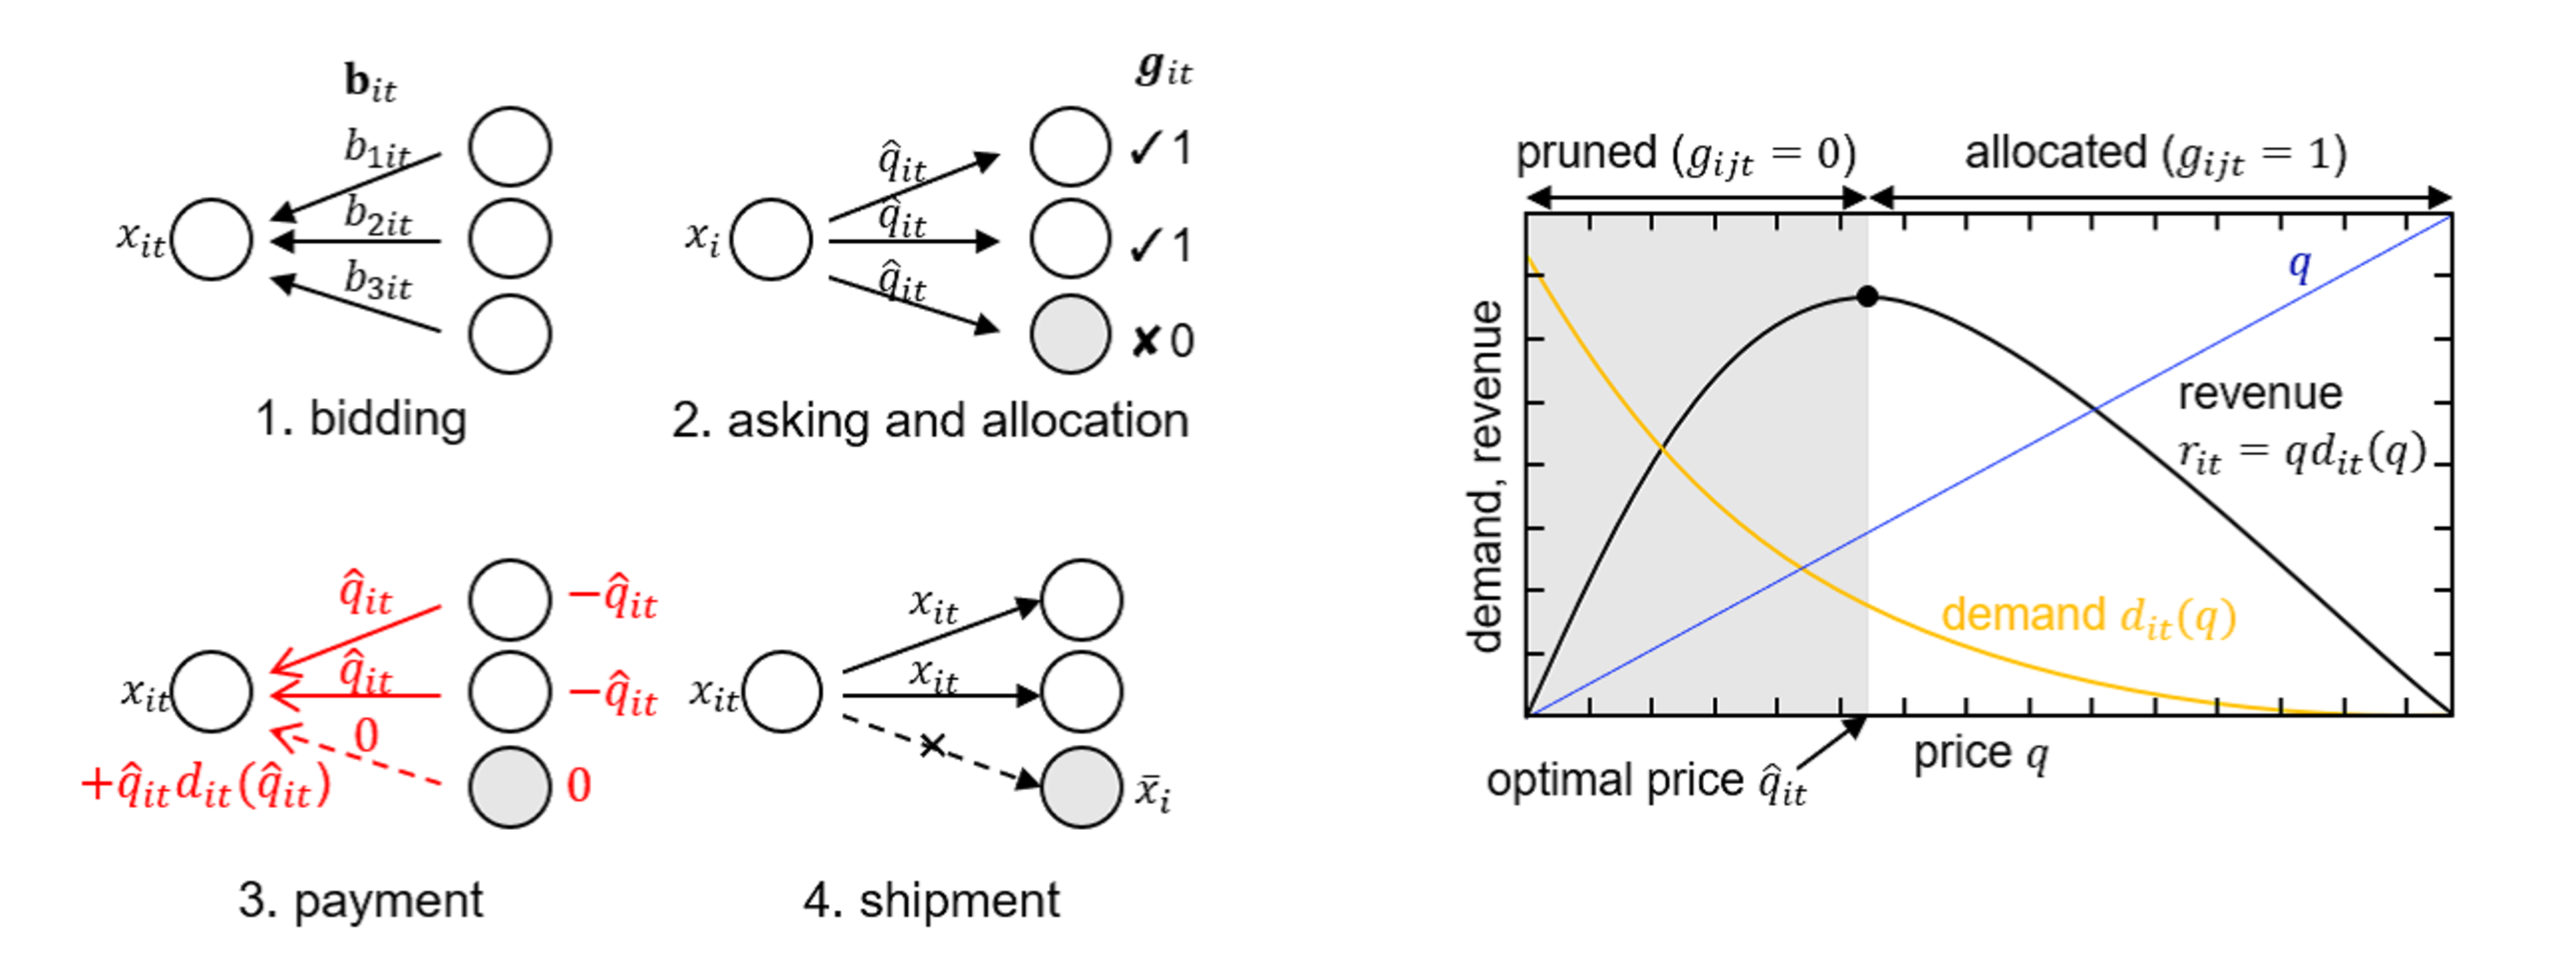
\includegraphics[width=\linewidth]{img/double.eps}
\caption{
�{�����ł́Adigital goods auction �̘g�g�݂�p���āA��V�̍œK�z������������B
}
\label{fig:double}
\end{figure*}

����܂ł̃j���[�����l�b�g���[�N�̖ړI�́A�\���덷 $e$ �ɂ������B
���̂��߁A�e���j�b�g�̓o�b�N�v���p�Q�[�V�����ɂ���� $\partial e / \partial y$ ���󂯎��A
$e$ ���������Ȃ������ $y$ �̑傫���𐧌䂵�Ă����B
NaaA �ɂ����āA�G�[�W�F���g�̖ړI�͑��I�덷�̍ŏ����ł͂Ȃ��A�G�[�W�F���g���g�̗��v�̍ő剻�ł���B
�����ŁA���v�Ƃ́A�G�[�W�F���g���󂯎�锄��ƁA�x�����R�X�g�̍��ł���B
���Ȃ킿�A�e�G�[�W�F���g�͎��̊֐����ő剻����B
\begin{flalign}
R_t = r_t - c_t
\end{flalign}

�G�[�W�F���g�̖ړI�֐��͎��̂悤�ɕ\�������B
\begin{flalign}
\Expect{\pi}{\sum_{i=0}^{T} \gamma^i (r_{t+i} - c_{t+i})}
&= \Expect{\pi}{\sum_{i=0}^{T} \gamma^i r_{t+i}} -  \Expect{\pi}{\sum_{i=0}^{T} \gamma^ic_{t+i}} \\
&= G_t^{\mathrm{in}} - G_t^{\mathrm{out}}
\end{flalign}
�������A$G_t^{\mathrm{in}} \equiv \Expect{\pi}{\sum_{i=0}^{T} \gamma^i r_{t+i}}$�A
$G_t^{\mathrm{out}} \equiv \Expect{\pi}{\sum_{i=0}^{T} \gamma^ic_{t+i}}$ �ł���B
���̎��́A�G�[�W�F���g���I�[��Ԃ܂łɐ��ݏo�����t�����l�ɓ������B
������s�����߂ɁA�G�[�W�F���g�͔���̍ő剻�ƃR�X�g�̍ŏ����𓯎��ɍs�����Ƃ��킩��B

���̎���ʏ�̘g�g�݂ɉ����ĉ����ƁA�R�X�g�ŏ����ɂ���ăG�[�W�F���g�͑��̃G�[�W�F���g�ɑ΂��ċ��z���x����Ȃ����Ƃ������ƂȂ�B
���̂��߁A���ׂẴG�[�W�F���g���t���[���C�_�[�ƂȂ�A�S�̂Ƃ��Ă̕�V��������Ƃ����A�p���[�g��ʖ�肪��������B
NaaA �ł͂����������邽�߁A�I�[�N�V�����̎d�g�݂�p���āA�������j�b�g�̏o�͐�ɂ��郆�j�b�g�����������邱�Ƃɂ���čœK���i�����肷��B

������P�������邽�߂ɁADQN �̂悤�� $l$ �w����Ȃ�t�B�[�h�t�H���[�h�l�b�g���[�N���l����B
�Ȃ��A�C�ӂ�DAG �\���i���ԕ����ɓW�J���ꂽ RNN ��z�b�v�t�B�[���h�l�b�g���[�N�j�ł����l�̂��Ƃ��l�����邽�߈�ʐ�������Ȃ��B
�e�G�[�W�F���g���󂯎���V�̑��a�͂��‹����^�����V�ɑ΂��ē������K�v������B���Ȃ킿�A���̎�����������B
\begin{flalign}
R_{S,t} = \sum_{i \in S} R_{it}
\end{flalign}
�œK�ȕ��z���@�Ƃ��Ă͂����‚��l�����邪�A�����ł͌n�S�̂���G�[�W�F���g����菜�����ꍇ�̊��ґ��� $D_{it}$ �ɂ�$R_{it}$ ���߂Â���Ƃ������@�����\cite{needed}�B
���̕��@�ł́A���ׂẴG�[�W�F���g���Ɨ��ɕ�V�ɍv�����Ă���ꍇ�ɁA$ \sum_{i \in S} D_{it} = R_{S, t}$ ����������

����́A��������Ƃ��āA��V�͐M�����m�̎���ɂ���ė^������Ƃ������̂�������B	% �V����I�B�Ȃ������邩�̐������Ȃ��Ă��Ȃ��B
���������āA�j���[�����́A�����ŁA�A�N�`���G�[�^ 0 �Ɛڑ����Ă��镡���̃��j�b�g�W�� $F_0 \subset S$ ���l����B
���̎��A�A�N�`���G�[�^�͓���ꂽ��V�̂����A���̂悤�ɂ��Ċe�m�[�h�ւ̕��z���s���B
\begin{flalign}
R_{0t} = \sum_{i \in V_0} r_{it}
\end{flalign}
�������A$r_{it}$ �͍v���x�ɉ�������V�z�ł���B
���ɁA���j�b�g $i$ �͌v�Z�ɕK�v�ȃf�[�^���u�w���v���邽�߂ɁA�ڑ�����Ă���i���Ȃ킿 $V_i$ �Ɋ܂܂��j���̃��j�b�g�ɑ΂��āA��V�����̂悤�ɂ��ĕ��z���邱�Ƃ��l����B
\begin{flalign}
c_{it} = \sum_{j \in V_i} r_{jt} + \alpha_{jt}
\end{flalign}
�������A$\alpha_i$ �� $c_{it}$ ���{���I�ɔ����Ă���R�X�g�i�ϑ��R�X�g�A�v�Z�R�X�g�j�ł���B
���̎d�g�݂��ċA�I�ɌJ��Ԃ��A���͑w�܂ŌJ��Ԃ��ƁA���̎�����������B
\begin{flalign}
R_{0t} = \sum_{i \in V_0} r_{it} = \sum_{i \in S} (r_{it} - c_{it}) 
\end{flalign}
���������āA$R_{it} = r_{it} - c_{it}$ ����������B
%����́A��V�͂��ׂẴm�[�h���A���ʂ̃��j�b�g����󂯎�����M���ɑ΂��ė^�����t�����l�̍��v�ɓ������B
���̎��́A$R_{0t}$ �́A�e���j�b�g�����ݏo�����t�����l $r_{it} - c_{it}$ �̍��v�Ƃ��ĕ\������邱�Ƃ��Ӗ����Ă���B

���̕t�����l�̂��Ƃ��ANaaA �ł͌o�ϊw�̃��^�t�@�[��p���āA���v(profit)�ƌĂԁB
���v�͋����w�K�ɂ����ĒNj��̑ΏۂƂȂ��V(reward)�ɑ�������B
���l�ɁA$r_t$ �����v(revenue)�A$c_t$ ���R�X�g(cost)�ƌĂԁB
���Ȃ킿�ANaaA �̘g�g�݂ł́A�e�G�[�W�F���g�͗��v�̍ő剻��ړI�Ƃ��āA���v�ő剻�ƃR�X�g�ŏ����𓯎��ɍs�����ƂɂȂ�B

�ʏ�̃j���[�����l�b�g���[�N�̘g�g�݂�p���čœK�����s���ƁA
���ׂẴG�[�W�F���g���x�����R�X�g�� 0 �Ɏ�������B
���������āA���̍œK�����̎����ȃi�b�V���ύt���Ƃ��ē�����̂́A
���ׂẴ��j�b�g�ɑ΂����V�� 0 �ł���A�A�N�`���G�[�^�[�݂̂���V���l������Ƃ����󋵂ł���B
����͔F�m����͂��y�������]���̏󋵂ƍ��v����B

�]���͂���ł��悩�������A���͂ɃR�X�g��������ꍇ�A�p���[�g��ʂȏ󋵂�������B
���Ȃ킿�A���̓��j�b�g�ɑ΂��ĕ�V���^�����Ȃ��ƁA���͑��̃C���Z���e�B�u���Ȃ��Ȃ�A$R_{it} = -\alpha_{it}$ �ƂȂ�B
���̏ꍇ�A���̓��j�b�g�͊ϑ������Ȃ������悢�Ƃ������f�ɂȂ�A�o�͂��~����B
���̌��ʁA�A�N�`���G�[�^�[���ł́A�s���̌���ɕK�v�ȃf�[�^�������킽��Ȃ��Ȃ�A��V���Ⴍ�Ȃ�B
���������󋵂�����邽�߂ɁA���ҕ�V�����ł���ꍇ�A�G�[�W�F���g�͍s�����Ȃ��B

���������邽�߂ɁANaaA �ł̓I�[�N�V�����̎d�g�݂�p���Ď����̍œK�z�����s���B

%���������āA���̎�����������K�v������B
%�����ό`����ƁA���̂悤�ɂȂ�B
%\begin{flalign}
%R_{jt} = R_{Nt} - \sum_{i=1, i \ne j}^n R_{it} = R_{Nt} - R_{N-\{j\}, t}
%\end{flalign}
%�����I�ɂ́A$R_{jt}$ �� N ���� $j$ ���������n�œ������V�ɓ��������߁A�G�[�W�F���g $j$ ���^����t�����l�Ƃ��ĂƂ炦�邱�Ƃ��ł���B
%\begin{flalign}
%\sum_{i=1}^n r_{it} = \sum_{i=1}^n c_{it}
%\end{flalign}

%g% �����قȂ邩
%gNaaA �ɂ����郆�j�b�g������܂ł̃��j�b�g�ƈقȂ�_�́A
%g���j�b�g�Ԃ̒ʐM���M���̈���I�ȗ���ł͂Ȃ��A����A
%g���Ȃ킿�M���Ǝ����̌����ł���_�ł���B
%g%���j�b�g�����̃��j�b�g����M�����󂯎��ۂ́A�����𕥂��K�v������B
%g
%g�������ȒP�ɂ��邽�߂ɁA�ŏ��� 2 �‚̃��j�b�g�ō\������锄���-�����胂�f��(seller-buyer model)���l����B
%g���̃��f���́A�����̃��j�b�g���M�����v�Z���A�v�Z�����l�ɑ΂��Ēl�i��t���Ĕ�����ɑ΂��Ē�(ask)����B
%g������́A���承�i����D(bid)����B�����A��]���i(ask price)�����D���i(bid price)�������΁A��]���i�Ɠ��D���i�̊Ԃ̉��i�ō��ӂ��A������͔����ɑ΂��ĉ��i���l����B
%gSeller-buyer ���f���̖��́A�����肪�l�؂�Ă��܂����Ƃł���B
%g����͑ΐ헪���������Ȃ��ƌĂ΂��B
%g��]���i�����肷�鍪���������Ȃ��_�ɂ���B
%g
%gNaaA �ł́A���j�b�g�̏o�͂��A�f�W�^�����A���Ȃ킿�A�����������ɑ��݂�����Ƃ݂Ȃ��������̍œK�z���ɂ‚��čl����B
%g���J�j�Y���f�U�C���ł́A�‹��� $(N, \Theta, 0)$ �ŕ\�������B
%g
%g�����ŏd�v�Ȃ̂́A�œK�ȉ��i�̌�����@�ł���B
%g���ɁA��‚̃��j�b�g�ƕ����̃��j�b�g����Ȃ郂�f���Aseller-buyers ���f�����l����B
%g��‚̃��j�b�g�́A�����̃��j�b�g�ɑ΂��āA���𔄂�B
%g
%g���j�b�g�͓��̓��j�b�g�ɑ΂��āA
%g����́A���j�b�g�͑��̃j���[�����ɑ΂��Ē艿
%g�o�͒l�́A���̃��j�b�g�ɑ΂��Ă��̃��j�b�g�̒艿 $a_it$ �Ŕ��p����
%g���������āA

%========================================
% ����
%========================================

�����ŁA����ƃR�X�g�̑I����@�ɂ‚��ĕ����Đ������s���B
�܂��A����ɂ‚��čl����B�G�[�W�F���g�͗��v���ő剻���������߁A���v�͎��̂悤�ɂ��ė^������B
\begin{flalign}
	r_{it} = \max_{ a \ge 0 } a d_t(a) 
\end{flalign}
�����ŁA$a$ �͉��i�A$d_t(a)$ �̓��j�b�g $i$ �̐M���ɑ΂��鉿�l�� $a$ �ȏ�ƕ]�����Ă���G�[�W�F���g�̐��ł���A���v(demand)�ƌĂԁB
���l�̎��ŁA�E�ӂ��ő剻���� $a$ ���œK���i�ƌĂсA$ \hat{a}_{it} $ �ŕ\���B 


%========================================
% �R�X�g
%========================================

���ɁA�R�X�g�ɂ‚��čl����B
�G�[�W�F���g�����̃G�[�W�F���g�ɑ΂��Ďx�����R�X�g�́A
�w���ɐ��������ꍇ�͔����̒񎦉��i $\hat{a}_{it}$ ���x�����A
�����łȂ��ꍇ�͎x�����R�X�g�� 0 �ɂȂ�B
�R�X�g�ŏ����̘g�g�݂���l����ƁA�x�����R�X�g�� 0 �ł��������I�Ԃ��Ƃ����邪�A
�G�[�W�F���g�͏�Ƀf�[�^���w�����Ȃ��I��������”\��������B
�������A����͐��ݓI�ɂ͏����̔���グ���������Ă��邱�ƂɂȂ�B
�f�[�^���w�������A�򈫂ȃf�[�^�𗬂����ꍇ�̔���̒ቺ���l����B
����́A�������f�[�^���w�������ꍇ�Ƃ����łȂ��ꍇ�̒��� $r_{it}$ �̍��ɓ������B
���Ȃ킿�A
%FIXME ���������͊��Ғl����Ȃ��ă��^�[�����̂��̂Ȃ̂ł��̂悤�ɏC������i�ŏ��Ƀ��^�[�����g�������W�b�N�Ő������Ă��邽�߁j
\begin{flalign}
	o_t 
	&= \Expect{\pi}{ r_{i,t+1} \mid a_t=1 } - \Expect{\pi}{ r_{i,t+1} \mid a_t=0 } \\
	&= \Expect{\pi}{ R_{i,t+1} \mid a_t=1 } - \Expect{\pi}{ R_{i,t+1} \mid a_t=0 } \\
	&= Q(s_t, 1) - Q(s_t, 0) \label{eq:def:oppotunity-cost},
\end{flalign}
�������A$Q$ �͏�ԍs�����l�֐��ł���A����̃R�X�g�͂ǂ���̍s����I��ł����ł���Ɖ��肵�Ă���B
$o_{it}$ �� counterfractual state-action value �ƌĂԁB����� QUICR \citep{agogino2006quicr} �Ɠ��o�͈قȂ邪�����ł���B
���Ȃ킿�A�G�[�W�F���g���x�����R�X�g�́A�f�[�^�̍w���ɐ��������ꍇ�� $\hat{a}_{it}$ �ł���A
����ȊO�� $o_{it}$ �ƂȂ�B

�ł́A�R�X�g���ŏ������邽�߂̃G�[�W�F���g�̓��D�z $b_{it}$ �͉����B
����ɂ‚��Ă͎��̒藝����������B

\begin{thm}\label{thm:optimal-bidding}
�R�X�g���ŏ�������œK�ȓ��D�z�� $b_{it} = o_{it}$ �ł���B
\end{thm}
�ؖ��ɂ‚��Ă� Appendix ���Q�ƁB

���Ȃ킿�A�G�[�W�F���g�͎��g�̋@����݂̂���ɂ���΂悢(!)
���������āANaaA �̃��J�j�Y���ł́A�G�[�W�F���g�͂����������̃G�[�W�F���g�����l�]��(valuation)���A
���̉��l�𐳒��ɐ\�����Ă��邱�Ƃ��Ӗ�����B

�n�Ƃ��Ď��̉���������B
\begin{coro}\label{coro:optimal-bidding}
The Nash equivalem of the envy-free game $(\vect{b}, q)$ is $(\vect{o}_t, \max_{q} q d_{\vect{o}_t}(q))$.
\end{coro}

%TODO o_t �̃O���E���h������B�ŏ��ɖ]�܂����z�� v ���q�ׁA���̌�ŏd�v���ɂ‚��ĉ������B


\subsection{Valuation Net}

\begin{figure*}[t]
\centering
\includegraphics[width=\linewidth]{img/network.eps}
\caption{
Valuationn Net �͏��̉��l��]�����Abidding price �����肷��B
���ʂ̃j���[�����ɑ΂��ē��D���A�M�����w������B�w�������f�[�^��p���āA�f�[�^�����̃j���[�����ɑ΂��Ĕ���B
}
\label{fig:network}
\end{figure*}

�c����́A$\vect{o}_t$ �������ɐ��肷�邩�ł���B
���̐���ɂ͗l�X�ȕ��@�����݂��Ă���A�����̃��\�b�h���g�����Ƃ��ł��邪�A
�{�_���ł� $Q$ �̐���� $Q$-learning ���̗p����B
�������ASARSA �� actor-critic �Ȃǂ� on-policy �ȕ��@���g�����Ƃ��ł��邱�Ƃ�⑫����B

�}\ref{fig:network}�Ɏ���Valuation Net �́A�ʏ�̃j���[�����l�b�g���[�N�̃��j�b�g�ɁA
$Q$-learning �ɂ�� valuation ��g�ݍ��킹���l�b�g���[�N�ł���B
�܂��A�㕔�̓G�[�W�F���g�Ԃ̒ʐM�ɂ‚��Ď��������̂ł���B
�j���[�����l�b�g���[�N�ł̓��j�b�g���~�ŕ\������̂��ʗ�ł��邪�A
�����ł̓��j�b�g���G�[�W�F���g�Ƃ��Ă݂Ȃ����Ƃ��������āA�Z�p�`�ň�‚̃��j�b�g��\�����Ă���B
�G�[�W�F���g�Ԃł́A�ʏ�̃j���[�����l�b�g���[�N�Ɠ��l�̐M���̒ʐM�ȊO�ɁA
����Ɋւ���ʐM(allocate, buy, sell \& bid)����������B

Valuation Net �ł́A��� $\vect{s}_t$ �Ƃ��āA
�\������� $\tilde{\vect{x}}_t$ ����ѓ��͂Ɉˑ����Ȃ��\����� $\vect{u}$ �����ɂ‚Ȃ����x�N�g�� $(\tilde{\vect{x}}_t^\T, \vect{u}^\T)^\T$ ��p����B
�\�����̈��Ƃ��Ă̓��j�b�g�̃p�����[�^���������A���Ƃ��Ώd�݂�o�C�A�X�̏���p���邱�Ƃ��ł���B

��Ԃ���� Q �֐��̗\���Ƀj���[�����l�b�g���[�N��p����B
�G�[�W�F���g���󂯎��������Ɋ�Â����ԍ���(TD)-�덷 ���v�Z����A
�l�b�g���[�N���P�������B
�l�b�g���[�N�̍\���ɂ͂���܂ł� deep Q-learning �ŗp�����Ă����d���l�b�g���[�N(dualing network) \citep{wang2015dueling} �̃e�N�j�b�N��p����B
�I���W�i���̕���\citep{wang2015dueling}�ŏq�ׂ��Ă����d���l�b�g���[�N�́A�w�K���������邽�߂ɁA
��Ԋ֐��ƁAQ�֐��Ƃ̍�����ʁX�ɗ\�������@�ł���B
\cite{dosovitskiy2016learning} �͂���ɑ΂��āA�����̗v�f�̑}�b�� 0 �ɂȂ�悤�ɐ��K������悤���ǂ��Ă���B
�{�����ł� \cite{dosovitskiy2016learning} �̎�@�ɏ]���A
���Ғl $E(\vect{s}_t)$ �Ɛ��K������ $\tilde{A}(\vect{s}_t)$ ��ʁX�ɋ��߂�B

$Q$�֐��͎��̂悤�ɕ\�������B
\begin{flalign}
	Q(\vect{s}_t, a_t) &= E(\vect{s}_t) + \tilde{A}(\vect{s}_t, a_t) \label{eq:QisE-A} \\
	\sum_{i+1}^k \tilde{A}_i(\vect{s}_t, a_t) &= 0
\end{flalign}
��2���𖞂������߂ɁA�܂��A$\vect{s}_t$�Ɋ�Â����\�����s���A���̂悤�Ȑ��K�����s���B
\begin{flalign}
	\tilde{A}_i(\vect{s}_t, a_t) &= A_i(\vect{s}_t, a_t)  - \frac{1}{k} \sum_{j=1}^k  A_j(\vect{s}_t, a_t)
\end{flalign}
���ɁAvaluation ���s���Abidding price $\vect{b}_t$ �����߂�B
$b_{it}$ �̒l�͎� \ref{eq:def:oppotunity-cost} ����ю� \ref{eq:QisE-A}���A�œK�ȓ��D���i $\hat{b}_{it}$ �͎��̂悤�Ɍv�Z�ł���B
\begin{flalign}
\hat{b}_{it} = \tilde{A}(\state_t, 1) - \tilde{A}(\state_t, 0)
\end{flalign}
Valuation Net �ł͂��̎��Ɋ�Â��Aadvantage �̏o�͂������Z���邱�Ƃœ��D���i���v�Z���Ă���B


%\subsection{Valuation Net}

% method


\section{Experiment}

\section{Discussion}
\subsection{Disadvantage}
Disdvantage としてまず挙げられるのは計算量である。
Envy-free auction では需要の計算にソートの演算が入るために、
直列化しなければならない箇所があるため、
これらについては近似を行うなどして改善していく必要がある。

個別の最適化技術について述べると、
Envy-free auction は、買い手のエージェント同士の価格がわからない sealed な状態であれば、
正直性(truthfulness)が成り立つが、一方で買い手同士がコミュニケーションを行い
価格を共有し合う状態においては、買い手が自由に価格を偽装できることが知られている。
これについては、によって解決方法が示されている。

Valuation Net は、用いるニューラルネットワークによっては実装が困難であることがある。
これは著者らの GitHub に Linear と CNN は公開しているが、
RNN などについては今後の研究課題となる。

\subsection{Application}
NaaA は、ネットワークが分散されている環境での学習や、サブモジュールでの制御に有用である。
具体的に、以下の技術に応用が可能である。

\begin{itemize}
\item ハイパーパラメータチューニング。Neuroevolution など、遺伝的アルゴリズムを用いてハイパーパラメータチューニングを用いるアルゴリズムがすでにいくつか提案されている。このとき、fitness 関数として利益を用いることで、より強化学習の目的に特化したニューラルネットワークを得ることができると考えられる。
\item アテンション制御。一部のアテンションの研究では、強化学習を用いてアテンションの制御を行っている。
\item アンサンブル。複数のモデルの混合に今回の技術を用いることができる。
\end{itemize}


\if0
(作成中)以下のトピックについて言及

何を観測するか考えるという意味合いにおいてはアテンションの拡張である

送金方法

通信スピードの問題

実際の POMDP への拡張

実装

オークションの competitive 性

\subsection{NaaA における「付加価値」とは何か}
具体的な付加価値の例は、統合( $\vect{w}^\T \vect{x}$ )、増幅・減衰( $cx$ )、整流( $\mathrm{ReLU}(x)$ )、バイアス ($x+b$) などである。

\subsection{信頼との関係}
\subsection{価値評価・買い物との関係}

\subsection{Disadvantage}
計算量の問題がある。

\subsection{アプリケーション}
NaaA は、分散環境で何かやったり、サブモジュールで何かコントロールするような場合に有用である。

・ハイパーパラメータチューニング(遺伝的アルゴリズムを用いてハイパーパラメータをチューニングする)
	・Neuroevolution。報酬系が fitness を決める。
・自己組織化ニューラルネットワーク
・アテンション制御
・アンサンブル法
\fi


\if0
想定される反論
・本質コストや NOOP の存在は、パレート劣位の証左にならない: オークションを使わなくても、最低コストだけ払えばよいのでは?
・
\fi


\section{Conclusion and Future Works}
�{�_���ł́APOMDP �̖��ݒ�ɂ����ėǎ��ȓ����\���𓾂邽�߂ɁA�j���[�����l�b�g���[�N��̊e���j�b�g���G�[�W�F���g�Ƃ��Ĉ����t���[�����[�N�ANaaA �ɂ‚��ďq�ׂ��B
NaaA �̃t���[�����[�N�ł́A�W�����}�����������A���ꂼ��̃G�[�W�F���g�̎��•t�����l���i�b�V���ύt�Ƃ��ē����A�S�̂Ƃ��ăp���[�g�œK�ɂȂ邱�Ƃ��������B
���D���i�̌���A���S���Y���̈�‚Ƃ��āA$Q$-learning �Ɋ�Â��l�b�g���[�N Valuation Net ���������B
�]�������ł́AAtari �� VizDoom ��p�����������s���A�������ʂ�������@�����悭�Ȃ邱�Ƃ��������B

% ����̕������͎v���‚����珑�������Ă���
����̕������Ƃ��āA�������AValuation Net �� A3C �Ȃǂ� on-policy �Ȏ�@�Œu��������Ƃ������������̑��A�_�o�Ȋw�I�Ȑ������”\�ɂ��Ă����Ƃ��������@�A��`�I�A���S���Y���Ƃ̑g�ݍ��킹����������B

\appendix
\section*{Appendix}

% Set numbering of section alphabet: A, B, C,...
\setcounter{section}{1}
\renewcommand{\thesection}{\Alph{section}}

% Contents is started from here
%\subsection{Proof}
%We first proof $\rho_{ijt} = 0$ is the Nash equilibrium.
%The value function can be written as $r_{it} - c_{it} + \gamma V_{i,t+1}$.
%At the point, as other agents plays $\rho_{ijt} = 0$, the value function is $- c_{it}$.
%To maximizing this equation, $\rho_{ijt} = 0$ holds. 

\subsection{Proof of Theorem \ref{thm:optimal-bidding}}
%As for a buyer, the asking price $\ask$ for a seller is unknown,
%we address $\ask$ which has support $[0, \infty)$,
%and consideration to maximize $\Expect{q}{G(b,q)}$,
%In this case, the following equation holds.
%\begin{flalign}
%\deriv{b}{}\Expect{q}{G(b,q)} 
%&= \deriv{b}{}\int_0^\infty (H(b - q) \cdot (v-q) + G_0) p(q) dq \notag \\
%&= \deriv{b}{} \left[ \int_0^b (v-q) p(q) dq + G_0 \int_0^\infty p(q)dq \right] \notag \\
%&= \deriv{b}{} \int_0^b (v-q) p(q) dq \notag \\
%&= (v-b) p(q=b), \notag 
%\end{flalign}
%Therefore, the condition to maximize $\Expect{q}{G(b,q)}$ is $b=v$.

The optimization problem in Eq:\ref{Eq:optimization-probem} is made of two terms except of the constant, 
and the only second term is depends on $\vect{b}$.
Hence, we consider to optimize the second term.
The optimal bidding prices $\hat{\vect{q}}_t$ is given by the following equation.

\begin{flalign}
\hat{\vect{b}}_{it} 
&= \argmin_{\vect{b}} \Expect{\vect{q}_t}{\vect{g}_{it}(\vect{b})^\T( \vect{q}_t - \gamma \vect{o}_{it}  )} 	
= \argmin_{\vect{b}} \Expect{\vect{q}_t}{H(\vect{b} - \vect{q}_{t})^\T ( \vect{q}_t - \gamma \vect{o}_{it}  )}	\notag \\
&= \argmin_{\vect{b}} \Expect{\vect{q}_t}{\sum_{j=1}^N H(b_{j} - q_{jt}) ( q_{jt} - \gamma o_{ijt}  )}		
= \argmin_{\vect{b}} \sum_{j=1}^N \Expect{q_{jt}}{H(b_{j} - q_{jt}) ( q_{jt} - \gamma o_{ijt}  )},
\end{flalign}

From independence, the equation is solved if we solve the following problem.

\begin{flalign}
\hat{b}_{ijt} = \argmin_{b} \Expect{q_{jt}}{H(b - q_{jt}) ( q_{jt} - \gamma o_{ijt}  )}, \, \, \, \forall j \in \{1, \dots, N\}
\end{flalign}

Hence, $\hat{b}_{ijt}$ can be derived as the solution which satisfies the following equation. 
\begin{flalign}
	\left. \deriv{b}{}\Expect{q_{jt}}{H(b - q_{jt}) ( q_{jt} - \gamma o_{ijt}  )} \right|_{b=\hat{b}_{ijt}}  = 0,  \, \, \, 
\left. \derivN{2}{b}{}\Expect{q_{jt}}{H(b - q_{jt}) ( q_{jt} - \gamma o_{ijt}  )}\right|_{b=\hat{b}_{ijt}} > 0 \notag 
\end{flalign}

For simplicity, we let $q = q_{jt}$ and $o = o_{ij,t+1}$. Then, the following equation holds.

\begin{flalign}
\deriv{b}{}\Expect{q}{H(b - q)( q - \gamma o  )} 
&= \deriv{b}{}\int_0^\infty H(b - q)(q - \gamma o) p(q) dq \notag \\
&= \deriv{b}{} \int_0^b (q - \gamma o) p(q) dq \notag \\
	&= (b-\gamma o) p(q=b), \label{eq:deriv1}
\end{flalign}
\begin{flalign}
	\derivN{2}{b}{}\Expect{q}{H(b - q)( q - \gamma o  )} = p(q=b) + (b - \gamma o) \deriv{b}{}p(q=b)  \label{eq:deriv2}
\end{flalign}

Then, condition $\deriv{b}{}\Expect{q_{jt}}{H(b - q_{jt}) ( q_{jt} - \gamma o_{ijt}  )} |_{b=\hat{b}_{ijt}}  = 0$ is satisfied only by $\hat{b}_{ijt} = \gamma o_{ijt}$.
We substitue $\hat{b}_{ijt}$ into Eq:\ref{eq:deriv2},
\begin{flalign}
\left. \derivN{2}{b}{}\Expect{q_{jt}}{H(b - q_{jt}) ( q_{jt} - \gamma o_{ijt}  )}\right|_{b=\hat{b}_{ijt}} 
	&= p(q=\hat{b}_{ijt}) + 0 > 0
\end{flalign}

Therefore, $\hat{b}_{ijt} = \gamma o_{ijt}$ is a unique solution as the minimum point.
From generality, $\hat{\vect{b}}_{it} = \gamma \vect{o}_{it}$ holds.


%%では、これらの活動がすべて異なる主体によって達成される場合がありうる。
%%・近年の深層強化学習の成功は、強化学習に深層学習を組み合わせることの有用性を示している。
%
%% 問題は何か
%現在主流となっている深層強化学習の枠組みでは、
%単一のエージェントが問題空間の観測、認知、行動決定のすべてを担う。
%
%%しかし、現実世界の問題では、観測、認知、行動決定がすべて異なる主体によって達成される場合がありうる。
%%分散化する知能は、近年様々な分野で言われている。
%%ビットコインは、多くの通貨する仕組みである。
%
%このように、重要である。
%実際、人間の脳は分散化されたニューロンによって構成される。
%この考え方はニューラルダーウィズムと呼ばれる。
%ニューラルダーウィズムの提唱者である***は、彼の著書の中でこのように語っている。
%
%本論文はニューロンを分散化した主体としてみなす。
%
%一つのニューロンを分散化することは容易ではない。
%なぜなら、ニューロンは報酬
%
%NaaA は、
%
%ここで見方を変えて、脳の中でどのようにニューロンの間の情報供給がなされているか見てみよう。
%ニューロンによる報酬系のやり取りは脳の中でも行われている。
%ニューロンには血管からグリア細胞を通して
%すなわち、有用な情報を提供しないニューロンは自死する仕組みが脳内にプログラミングされている。
%
%入力側のエージェントにとって、情報処理に見合う対価を得る必要がある。
%これまで成功してきた深層学習モデル(DQNやA3C)など、
%単一のエージェントモデルは、これらの問いを扱うことができない。
%
%なぜなら、センサー、モデル、アクチュエータのすべてが平等に報酬を受け取る必要がある。
%これは、信用割り当て問題と呼ばれる。
%
%現実の世界に適用する場合、よりスケーラブルに考える場合、
%分散型環境に適用したい。
%
%一方、
%
%% 考え方
%本論文では、
%エージェント同氏が通貨を使ってやり取りする。
%ゲーム理論に基づき、エージェントが最適な価値を評価できるようにする。
%これらは、実世界においてもビットコインなどの仮想通貨における送金が可能であるモデルである。
%
%% 実際のオークションの仕組み
%通貨の価値を最大化するため、NaaA はオークションの理論を用いる。
%
%% 
%本論文の貢献は以下の通りである。
%・信頼度割当問題を、個々のニューロンをエージェントとみなす手法を提案することで解決した
%・提案手法の有用性を、数値実験を用いて確認した。
%
%NaaA が提案する報酬系の枠組みは、
%近年のビットコインなどによる報酬系とも組み合わせることができる。
%そのため、社会実装を視野に入れたモデルである。

%すべてのユニットをエージェントとみなす方法は、マルチエージェント協力ゲームとして最適化を行う。

% 何の問題を解決するか
% ここをもう少し強化: 問題が何なのか説明され切れていない
% エネルギーに関する話も書く
%こうしたマルチエージェントの状況において、DQN や A3C などの単一エージェントを前提としたモデルはうまく動作しない。
%その理由の一つに最適な報酬分配の問題がある。
%どのように報酬を分配するのかという、マルチエージェント学習における信頼度割り当ての問題に帰着される。


\bibliography{daisy}
\bibliographystyle{iclr2017_conference}

\end{document}

